\documentclass[UTF8]{ctexart}

\usepackage{amsmath}
\usepackage{multicol}
\setlength{\parindent}{2em}
\addtolength{\topmargin}{-54pt}
\setlength{\oddsidemargin}{0.63cm}  % 3.17cm - 1 inch
\setlength{\evensidemargin}{\oddsidemargin}
\setlength{\textwidth}{14.66cm}
\setlength{\textheight}{24.00cm}    % 24.62
\usepackage{graphicx}
\usepackage{float}
\usepackage{multirow}
\usepackage{subfigure}
\begin{document}

%标题
\begin{center}
\huge\textbf{氦氖激光器横纵模分析及模分裂与模竞争}
\renewcommand{\baselinestretch}{5.0}
\end{center}
\begin{center}
\small
\begin{tabular}{llll}
\textbf{姓名}&李励玮     &\textbf{学号}  &201711140236\\
\textbf{指导老师}&王海燕 &\textbf{实验日期}& 2019.11.29\\
\end{tabular}
\end{center}

%摘要
\small
\noindent\textbf{摘要}:由于增益介质的存在,增益介质对不同频率的光的增益系数不同,有对应的增益曲线;在激光谐振腔中反射时增益大于损耗的频率的光才能出射,故激光器只能出射一定频率的光,这个频率范围就是出光带宽。激光谐振腔有本征频率,每一个频率对应一种光场分布,叫做一种模式,可以用纵模和横模来完整地描述出来。利用共焦球面扫描干涉仪可以得到激光器出射光的模谱,并对出射光的横、纵模对应的频率间隔进行计算。石英晶体的双折射现象可以使发生模分裂。
\newline\textbf{关键字:纵模、横模、模分裂、模竞争、增益曲线、出光带宽}

~\\

\begin{multicols}{2}

\section{引言}
激光器由增益介质、光学谐振腔和激励能源组成。激光谐振腔有本征频率,每一个频率对应一种光场分布,叫做一种模式。引进纵模和横模的概念,纵模描述轴向光场分布状态,横模描述横向光场分布状态,只要知道纵模和横模,则谐振腔内每个本征频率对应的光场分布状态就可以完整地描述出来。先讨论空腔,气体增益介质充入空腔后成为有源谐振腔,得到的模式结构与空腔一样,只有在谐振腔内往返一次增益大于损耗的光才能建立稳定的振荡,因此激光器输出的激光只包含少量的模式。

谐振腔的结构不同,它的模式也不同,实验中使用的共焦球面扫描干涉仪,测量激光的频谱间隔;结合激光的远场横向分布,可以分析激光器建立的激光的横模序数。

“偏振”是激光器输出光束的特性之一。相邻的两个纵模要么只可能是正交偏振或平行偏振的激光。模分裂指的是由物理效应(如双折射和塞曼效应等)把激光器的一个频率“分裂”成两个的现象。


\section{实验目的}
本实验研究由激光谐振腔本征频率及其对应的光场分布和双折射效应引起的激光频率分裂。通过观察激光器偏振、纵模、纵模分裂和模竞争等物理现象,加深学生对物理光学中的偏振、双折射以及激光原理中的频率(纵模)、出光带宽、激光烧孔和模竞争效应的理解。同时,让学生了解物理光学原理是如何与激光技术结合产生新现象的。

\section{实验原理}
\subsection{He-Ne激光器的纵模、横模及其对应的频率间隔}
激光器包括增益介质和光学谐振腔。使激光器的工作物质处于粒子数反转状态,自发辐射产生初始的光;光通过增益介质被放大,被反射镜反射后,再次通过增益介质被放大,多次往返,增益大于损耗的频率的光逐渐加强,最后在谐振腔中形成稳定的光场分布,便有激光输出。

\subsubsection{纵模}
在来回反射过程中,两列沿轴向相对传的同频率的光相干迭加形成驻波,当$2\mu L=q\lambda$驻波场稳定,该稳定驻波场为纵模。式中$\mu$为增益介质的折射率(气体介质$\mu\approx1$);$L$为谐振器长;$\lambda$为波长;$q$为纵模序数,为沿激光器轴线(z轴)场强为零的节点数。

\subsubsection{横模}
来回反射过程中,由于工作物质的横截面和镜面有限,当平行光通过它们时发生衍射,出射光波的波阵面发生畸变,从而在横向(即垂直于光的传播方向上),出现各种不同的场强分布。每种分布形式叫做一种横模。

横向分布是二维的,故可以用两个符号m、n标记,记作$TEM_{mn}$模,$m$表示沿x轴场强为零的节点数,$n$是沿y轴场强为零的节点数。

\subsubsection{频率间隔}
$TEM_{m,n,q}$可完善地描述一个模式,$\nu_{m, n, q}$表示对应的频率。纵、横模间隔是指纵、横模序数不同的本征模式之间的频率间隔。
\newline\textbf{(1)纵模间隔}:
\begin{equation}
\Delta \nu_{\mbox{纵}}=\nu_{m, n, q+\Delta q}-\nu_{m, n, q}=\frac{c}{2 \mu L} \Delta q
\end{equation}

$L$对不同的$m$、$n$虽然数值略有不同,但在所测精度范围内,相邻纵模频率间隔都相等。
\newline\textbf{(2)横模间隔}:

横模的频率间隔与谐振腔的二块反射镜的曲率半径及腔长有关,实验中所用的非共焦腔的横模频率差
\begin{equation}
\begin{aligned}
\Delta \nu_{\mbox{横}}&=\nu_{m+\Delta m, n+\Delta n, q}-\nu_{m, n, q}\\
&=\frac{C}{2 \mu L}\left\{\frac{1}{\pi}(\Delta m+\Delta n) \cos ^{-1}\left[\left(1-\frac{L}{R_{1}}\right)\left(1-\frac{L}{R_{2}}\right)\right]^{\frac{1}{2}}\right\}
\end{aligned}
\end{equation}
其中$R_{1}$和$R_{2}$为两反射镜的曲率半径。若腔长$L$比反射镜的曲率半径小,则横模频率间隔比纵模频率间隔小。

\subsection{He-Ne激光器纵模分裂及模竞争}
\subsubsection{石英晶体双折射效应}
石英晶体双折射效应使o光和e光具有光程差$\delta$。在不考
虑旋光性时,有
\begin{equation}
\begin{array}{l}{\delta=\left(n^{\prime \prime}-n^{\prime}\right) h} \\ {n^{\prime \prime}=\left(\frac{\sin ^{2} \theta}{n_{e}^{2}}+\frac{\cos ^{2} \theta}{n_{o}^{2}}\right)^{-1 / 2}} \\ {n^{\prime}=n_{0}}\end{array}
\end{equation}
其中$h$为晶片厚度,$n^{\prime}$和$n^{\prime \prime}$分别是o光和
e光的折射率,$n_{o}$和$n_{e}$分别是石英晶体的两个主折射率,$\theta$是石英晶体的晶轴和光线之间的夹角。故可以通过改変$h$和$\theta$的大小来改变和控制光程差$\delta$的大小。
\subsubsection{双折射效应产生纵模分裂及模竞争}
根据形成光驻波的条件,波长$\lambda$和激光腔总光程$L$应满足
\begin{equation}
L=\frac{\lambda}{2}q
\end{equation}
由式(4)可知$\nu=\frac{C}{2 L} q$,取微分得
\begin{equation}
\Delta \nu=-\frac{C}{2 L^{2}} q \Delta L=-\frac{\nu}{L} \Delta L
\end{equation}
$\Delta L$为谐振腔长的改变,$\Delta \nu$为由$\Delta L$引起的频率改变。

由于双折射元件,o光和e光在激光腔中的光程不同,所以原本唯一的谐振腔长“分裂”为两个腔长,两个谐振腔长有不同的谐振频率,即发生了频率分裂。把双折射元件引入的光程差$\delta$看作谐振腔长之差$\Delta L$,故得到
\begin{equation}
\Delta v=-\frac{v}{L} \delta
\end{equation}

\subsection{共焦球面扫描干涉仪}
\subsubsection{结构原理}
共焦球面扫描干涉仪由两共焦球面反射镜组成,其中一反射镜固定,另一反射镜固定在压电陶瓷环上。压电陶瓷环的长度将随外加电压的大小改变而变化,变化量与电压成正比。

共焦球面扫描干涉仪的光路图如图
\begin{figure}[H]
\centering
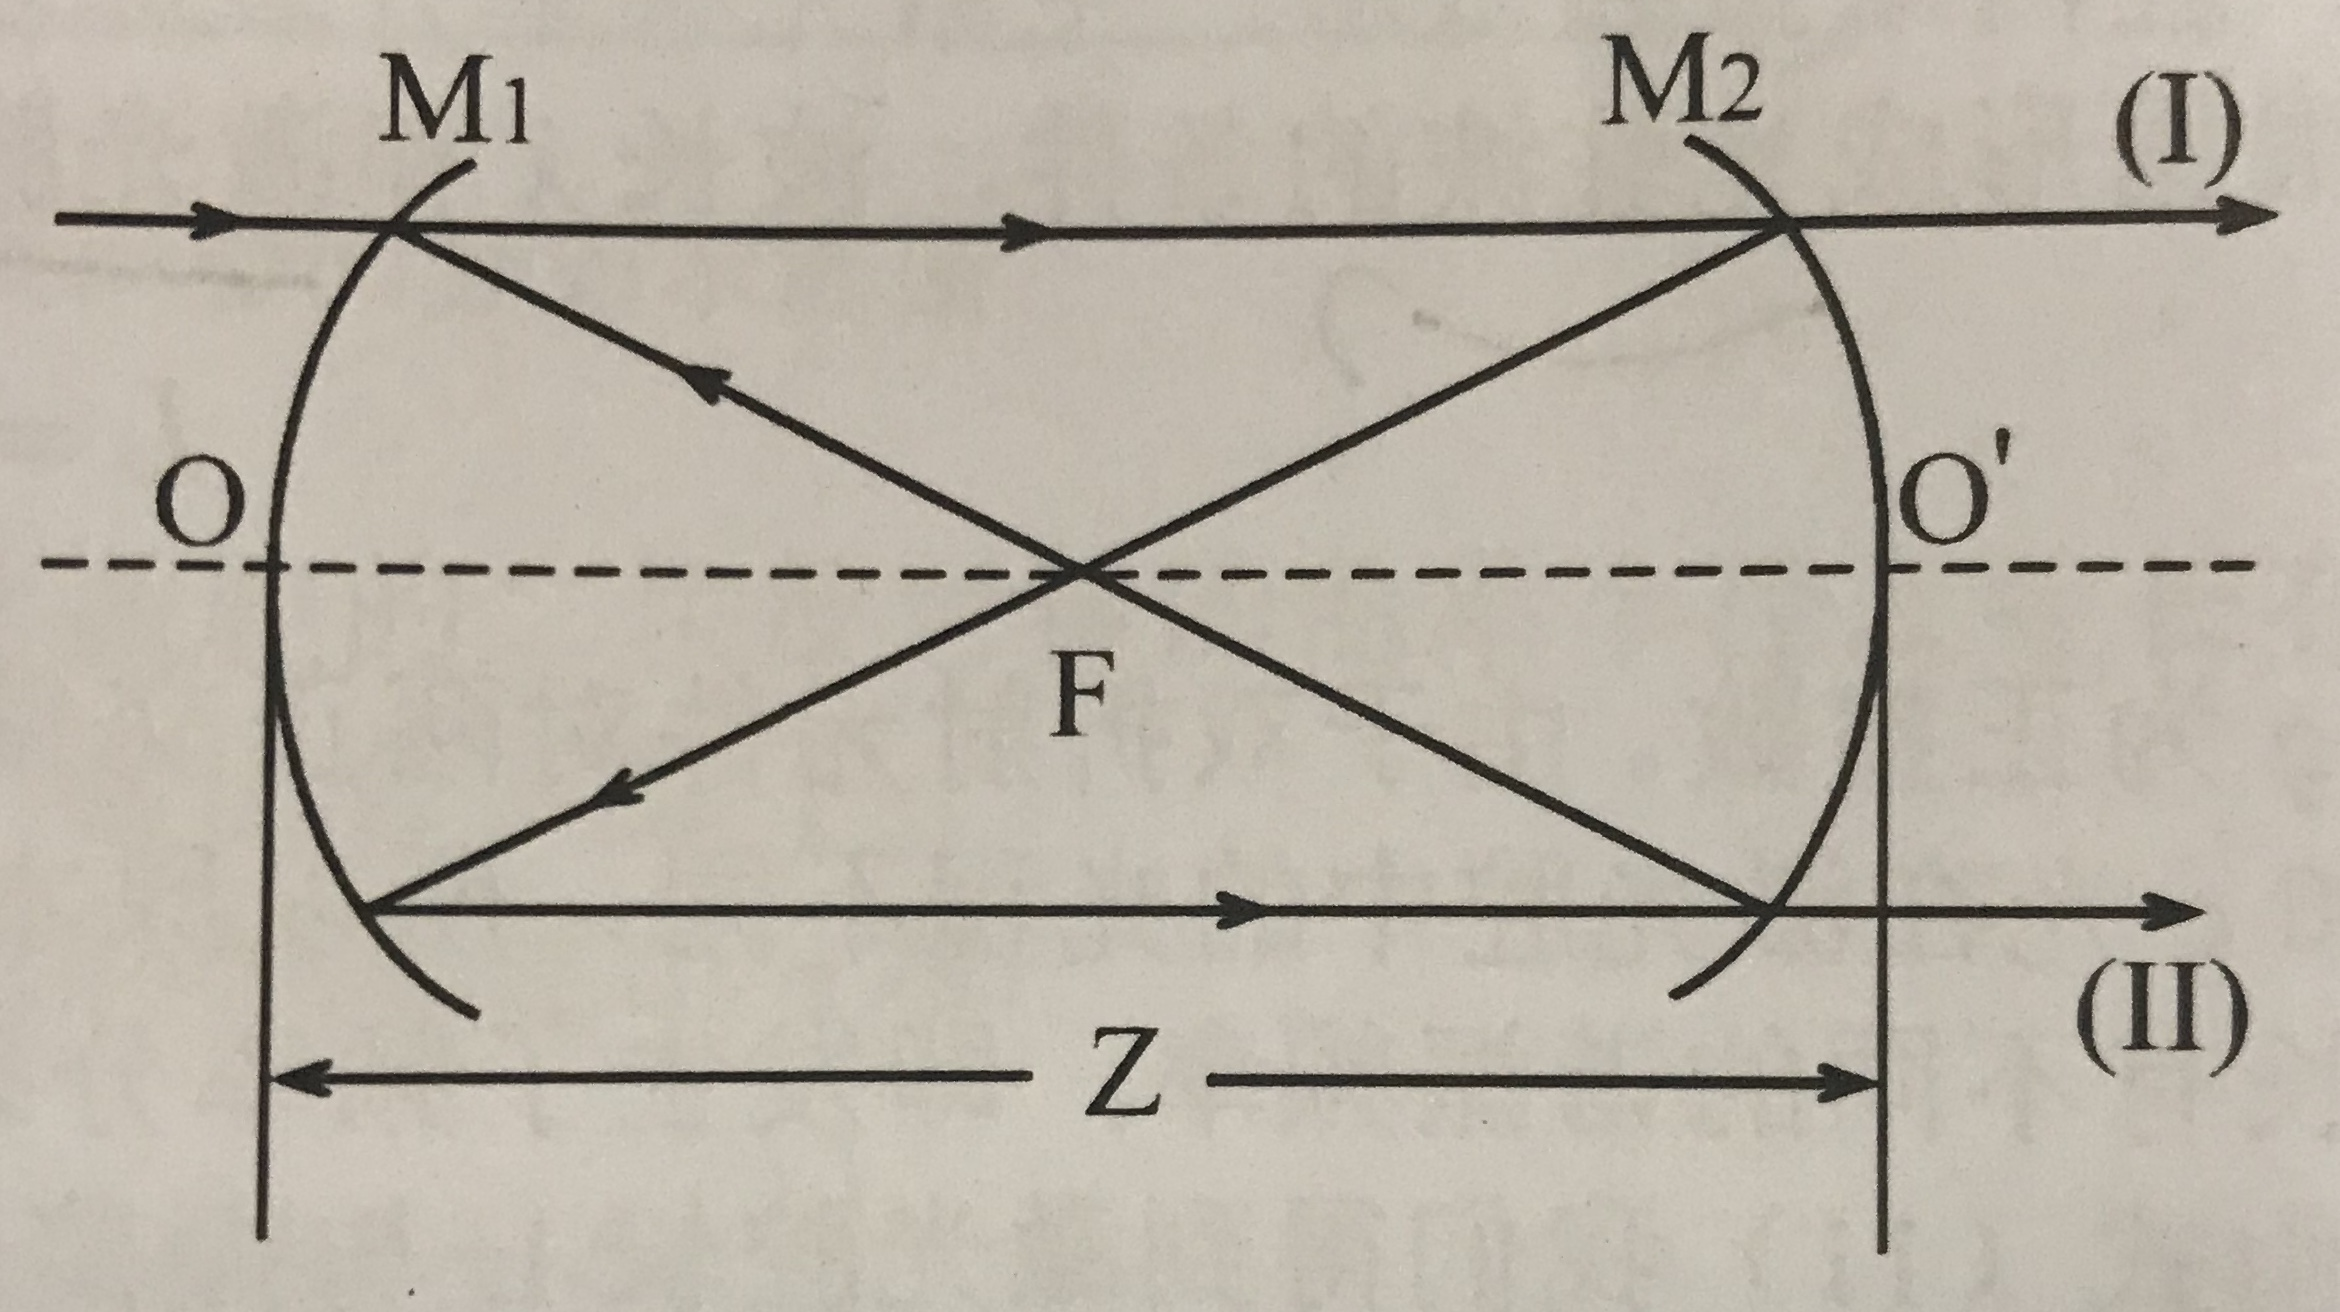
\includegraphics[width=5cm]{lightpath}
\end{figure}
可以看出,一束入射光有二组透射光,一组反射了$4m$次,另一组反射了$4m+2$次(Ⅱ型),如果相邻两束光的程差满足$\delta=4\mu L=K\mu\lambda$
其中$K$为整数(空气介质中$\mu=1$),则透射光束相干迭加产生干涉极大,故透过干涉仪的激光频率
\begin{equation}
\nu=\frac{c}{\lambda}=\frac{K c}{4 L}
\end{equation}
因为$L$是在所设计的腔长$L$附近作极微小的变化,于是有$L=L_{0}+\delta L$,代入式(7)展开并取一级近似可得$\nu=\frac{c K}{4 L_{0}}\left(1-\frac{\delta L}{L_{0}}\right)$,故可得
\begin{equation}
\Delta \nu=\nu-\nu_0=\nu-\frac{Kc}{4 L_{0}}=-\frac{Kc}{4 L_{0}^{2}} \delta L
\end{equation}
说明$\nu$的变化与腔长的变化量$\delta L$成正比,也就是与加在压电陶瓷环上的电压成正比。示波器的横向扫描采用与干涉仪的腔长扫描同步,示波器荧光屏上的横坐标就可表示干涉仪的频率变化。

\subsubsection{干涉仪的自由光谱区}
设原波长为$\lambda_1$、变化后波长为$\lambda_2$,当镜间距离的变化量$\delta L=\frac{\lambda_{1}}{4}$时,相当于干涉级次改变了1,则波长为$\lambda_1$及$\lambda_2$的光束同时透过干涉仪,两束光不可分辨,测量不再有意义。因此定义自由光谱区$\Delta\lambda_{SR}=\lambda_2-\lambda_1$。

由于$K \frac{\lambda_{2}}{4}=(K+1) \frac{\lambda_{1}}{4}$,计算得
\begin{equation}
\begin{array}{l}{\Delta \lambda_{S R}=\frac{\lambda^{2}}{4 L}} \\ {\Delta\nu_{S R}=\frac{c}{4 L}}\end{array}
\end{equation}

已知干涉仪的自由光谱区则可以标定横坐标频率变化的确切数值。

\subsubsection{扫描干涉仪的腔长设计}
为了把He-Ne激光器的所有频谱都在同一级光谱内显示,在设计扫描干涉仪的腔长时,
要使扫描干涉仪的自由光谱区$\Delta\nu_{S R}\geq$氮氖激光器工作波长的荧光线宽$\Delta\nu_{F}$。氨氖激光器632.8m的$\Delta\nu_{S R}=15\times10^9Hz$。

\section{实验内容}
\subsection{分别测量两根He-Ne激光管的模谱分布}
\noindent\textbf{1.在导轨的两个光具座上分别安装好激光管和扫描干涉仪}

激光管要轻拿轻放,安装时不可压得过紧。固定扫描干涉仪入口端的螺套要适当拧紧。激光管铝筒一侧为输出端,应对向扫描干涉仪入口端。取下扫描干涉仪端口的防尘盖。
\newline\textbf{2.用DW3型激光电源给激光管供电}

从电源后部红、黑插座引出的线分别接激光管的正、负极(铝筒端),千万不要接反
\newline\textbf{3.光路粗调}

接好线后打开激光电源和扫描干涉仪驱动电源。调整两个光具座使得从扫描干涉仪入口反射回到激光器输出端的光斑大体与激光束同心
\newline\textbf{4.光路细调}

打开放大器信号传输电源(开关在后部)及示波器电源。将光电探测器输出的信号经放大器放后输入示波器,仔细调整光路使得在示波器上看到的模谱信号为最大。
\newline\textbf{5.改变偏置电压、锯齿波幅度,观察这些因素对模谱的影响。}
\newline\textbf{6.测量激光管的相邻纵、横模频率间隔}

在示波器上确定扫描干涉仪自由光谱区范围,并据以测量模谱间隔。
\newline7.根据讲义中横模频率间隔公式结合观测横向光场分布,判断包含哪些横模。
\newline8.观察并记录一个自由光谱区的模谱图,并描绘模谱轮廓曲线。
\newline9.测量完成后,取下激光管放回包装盒。两根激光管都测完后,关闭所有电源。

\subsection{观测He-Ne激光器的纵模分裂和模竞争}
\noindent\textbf{1.搭建光路,连接仪器}

检査激光器与“氮氖激光器通用电源”和“压电陶瓷电源”的连接,取下激光器出光口防尘盖。将扫描干涉仪安装到激光器前面的光具座上。(激光管长详见各仪器)

打开激光电源,将“选择”置于Ⅱ,“粗调”由0拨至1,调整细调钮,使电流达到5mA。

打开“压电陶瓷电源”和“扫描干涉仪电源”
\newline\textbf{2.光路调整}

按照实验步骤(一)中第3步和第4步进行。
\newline\textbf{3.出光带宽观测}

改变加在压电陶瓷上的电压,模谱将在示波器上移动并改变幅值。记下谱线左边和右边消失点,二消失点的频率间隔即是出光带宽。并在这左右两个消失点中选测3-4个点,描出激光管增益曲线的大致轮廓。
\newline\textbf{4.激光偏振态的观测}

调整石英晶片晶轴与光束夹角,使纵模谱线产生足够的分裂间距。

在激光纵模分裂后,将偏振片置于激光器输出镜和扫描干涉仪之间,旋转偏振片,在示波器上观察两个分裂谱线的幅值变化情况,确定两分裂谱线间的偏振关系,并解释原因。
\newline5.实验完毕关闭所有电源,盖好激光器和扫描干涉仪的防尘盖。


\section{实验结果分析与讨论}
\subsection{改变偏置电压、锯齿波幅度对模谱的影响。}
改变偏置电压时锯齿波与模谱相对位置发生改变,模谱发生改变,说明干涉仪的$L_0$发生改变,而$\delta L$不改变,因此透过干涉仪的激光频率改变,引起模谱的变化。
\subsection{长管}
\subsubsection{激光管的相邻纵、横模频率间隔}
谐振腔长度$L=350mm$,自由光谱区为$2667MHz$,测得$\Delta t=3.960ms$。

当$\Delta q=1$时,计算得理论值
\newline $\Delta \nu_{\mbox{纵}}=\frac{c}{2 \mu L} \Delta q=428.57MHz$;

当$\Delta m+\Delta n=1$时,计算得理论值
\newline $\Delta \nu_{\mbox{横}}=\frac{C}{2 \mu L}\left\{\frac{1}{\pi}(\Delta m+\Delta n) \cos ^{-1}\left[\left(1-\frac{L}{R_{1}}\right)\left(1-\frac{L}{R_{2}}\right)\right]^{\frac{1}{2}}\right\}=86.36MHz$

\begin{figure}[H]
\centering
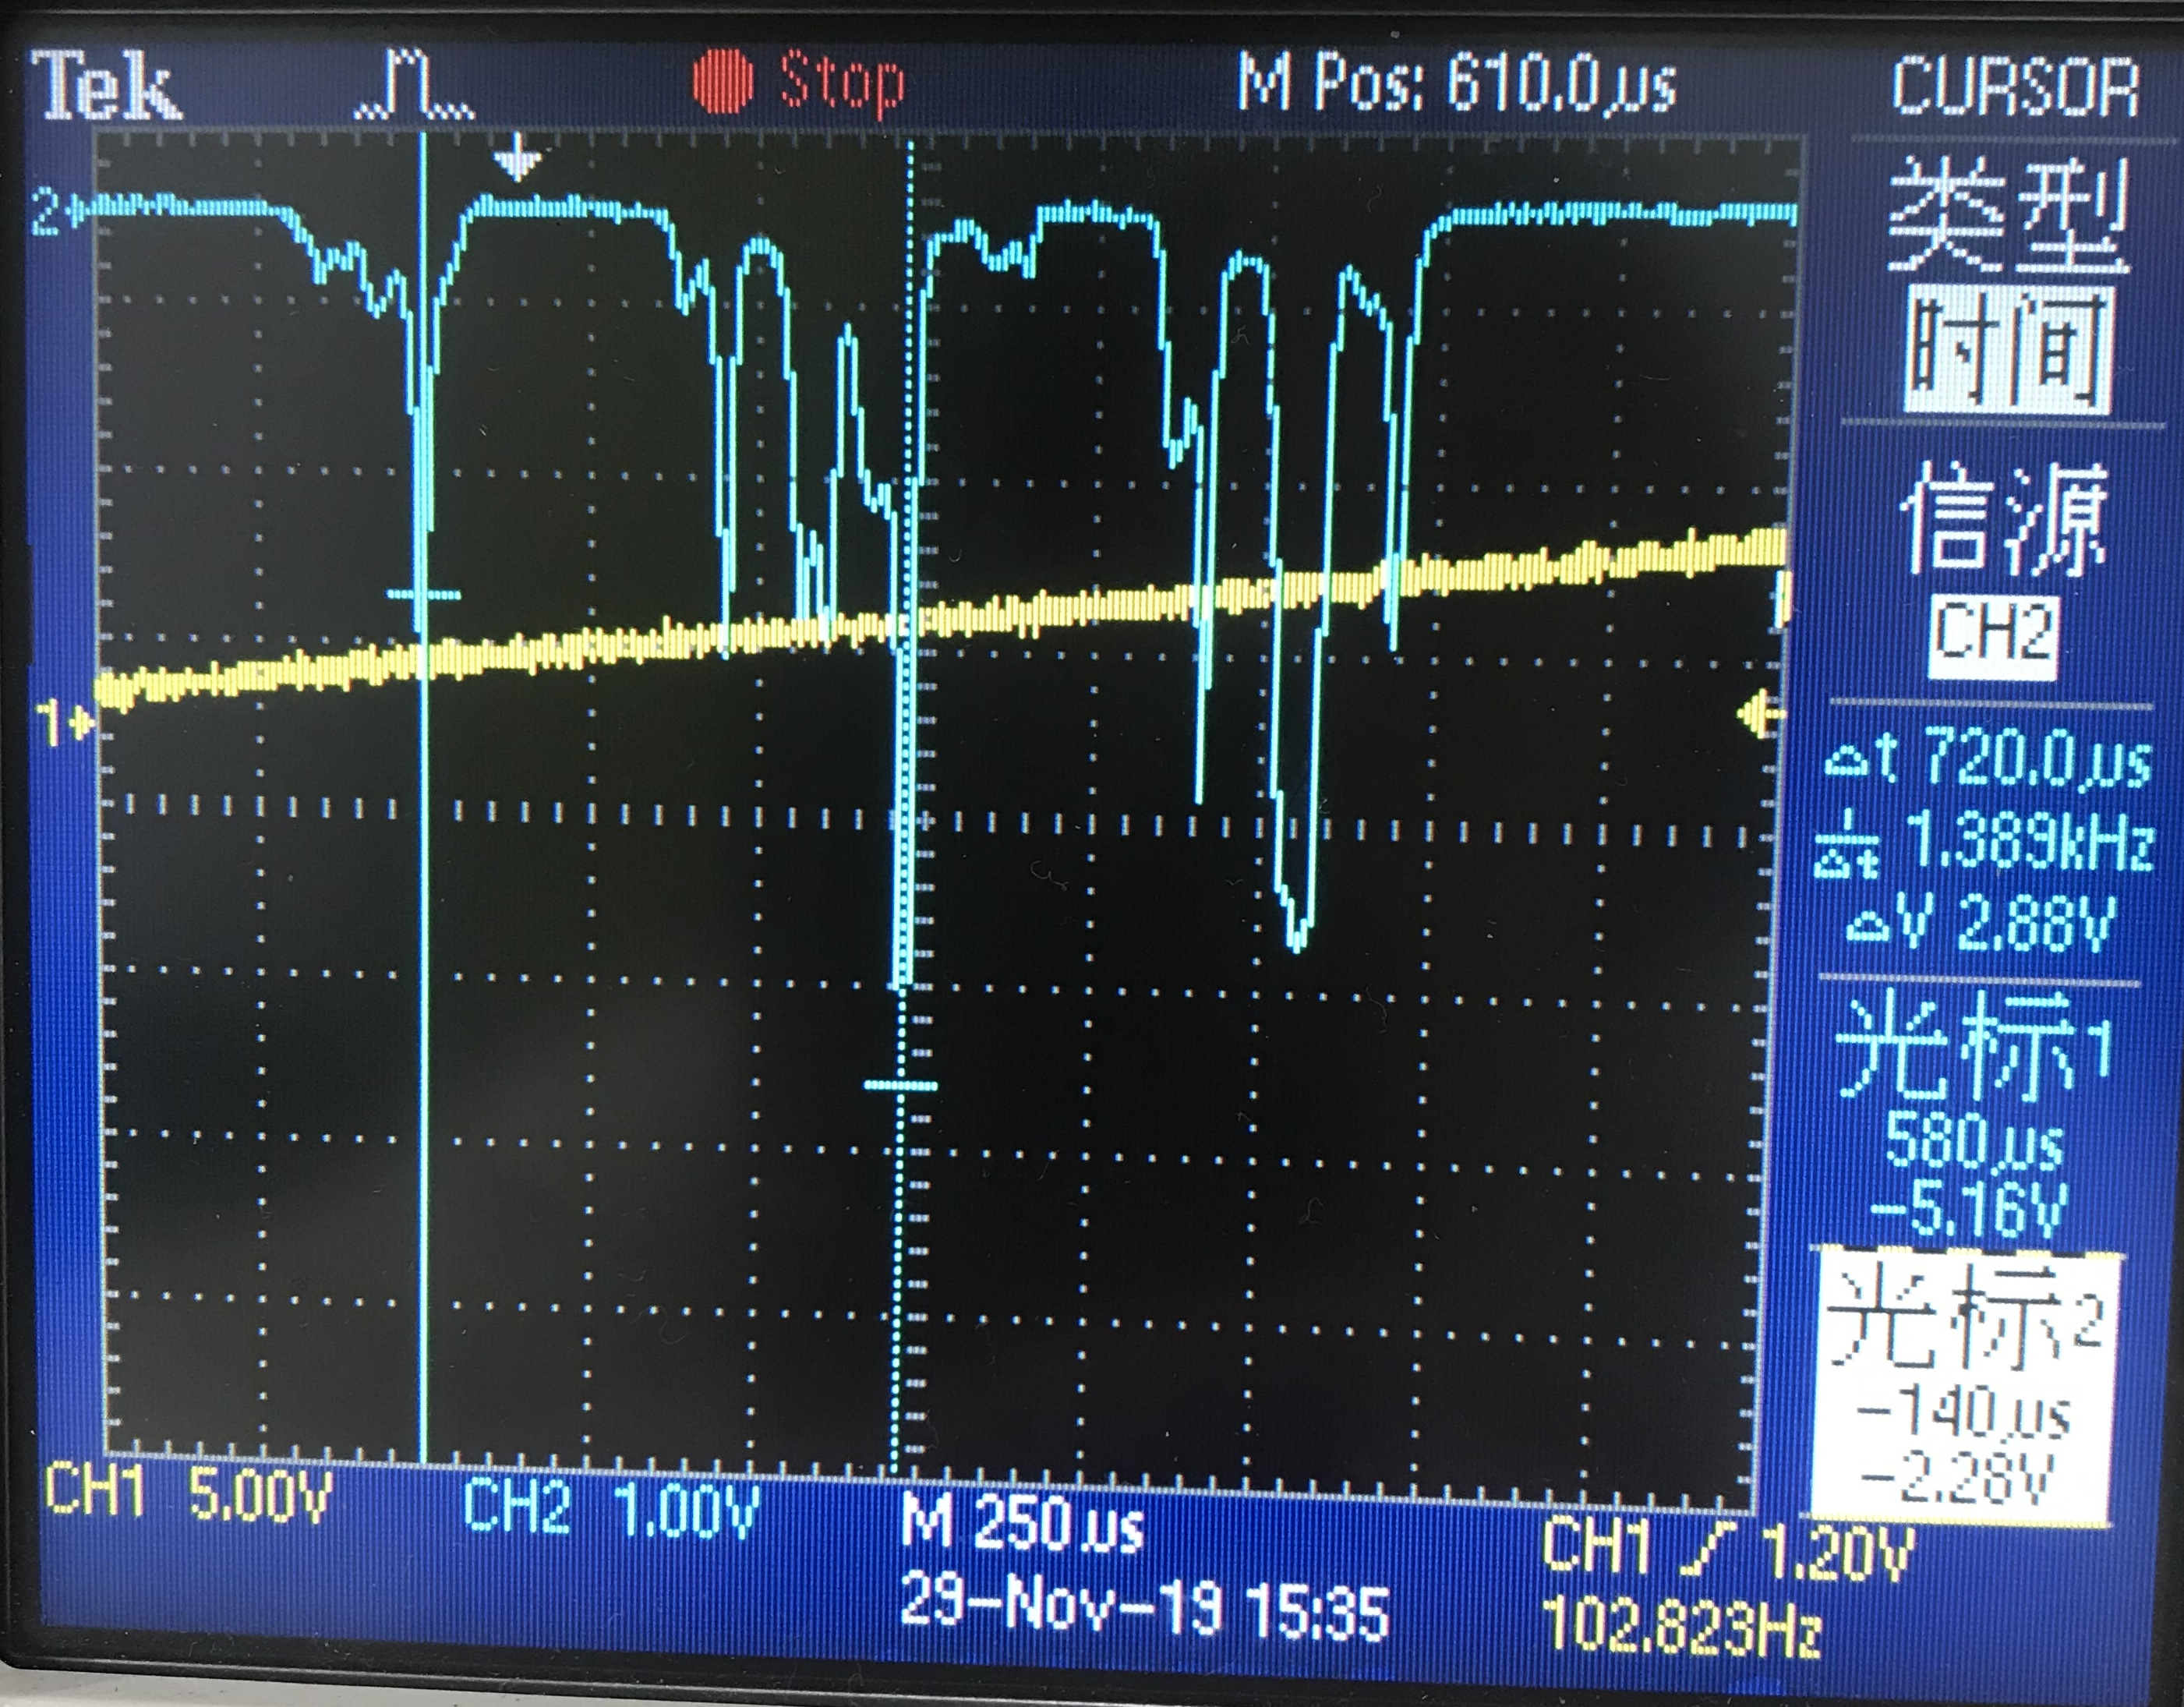
\includegraphics[width=6cm]{long-lengthways}
\caption{长管模谱图}
\end{figure}

观察模谱,可知有三个纵模,测得
\begin{table}[H]
\centering
\tiny
\begin{tabular}{|c|c|c|}
\hline
                 & 1     & 2     \\ \hline
$\Delta t/ms$ & 0.720 & 0.710 \\ \hline
\end{tabular}
\end{table}
平均$\overline{t}=0.715ms$,由自由光谱区大小可计算得
\newline$\Delta \nu_{\mbox{纵}}=0.715ms\times\frac{2667MHz}{3.960ms}=481.54MHz$

误差为$(481.54-428.57)/428.57\times100\%=12.4\%$。

有三个横模,测得
\begin{table}[H]
\centering
\tiny
\begin{tabular}{|c|c|c|c|}
\hline
                 & 1     & 2  &3   \\ \hline
$\Delta t/ms$ & 140 & 160 &150 \\ \hline
\end{tabular}
\end{table}
平均$\overline{t}=0.150ms$,由自由光谱区大小可计算得
\newline$\Delta \nu_{\mbox{纵}}=0.150ms\times\frac{2667MHz}{3.960ms}=101.02MHz$

误差为$(101.02-86.36)/86.36\times100\%=17.0\%$。

\subsection{短管}
\subsubsection{激光管的相邻纵、横模频率间隔}
谐振腔长度$L=242mm$,自由光谱区为$2667MHz$,测得$\Delta t=4.04ms$。

当$\Delta q=1$时,计算得理论值
\newline $\Delta \nu_{\mbox{纵}}=\frac{c}{2 \mu L} \Delta q=619.83MHz$。

\begin{figure}[H]
\centering
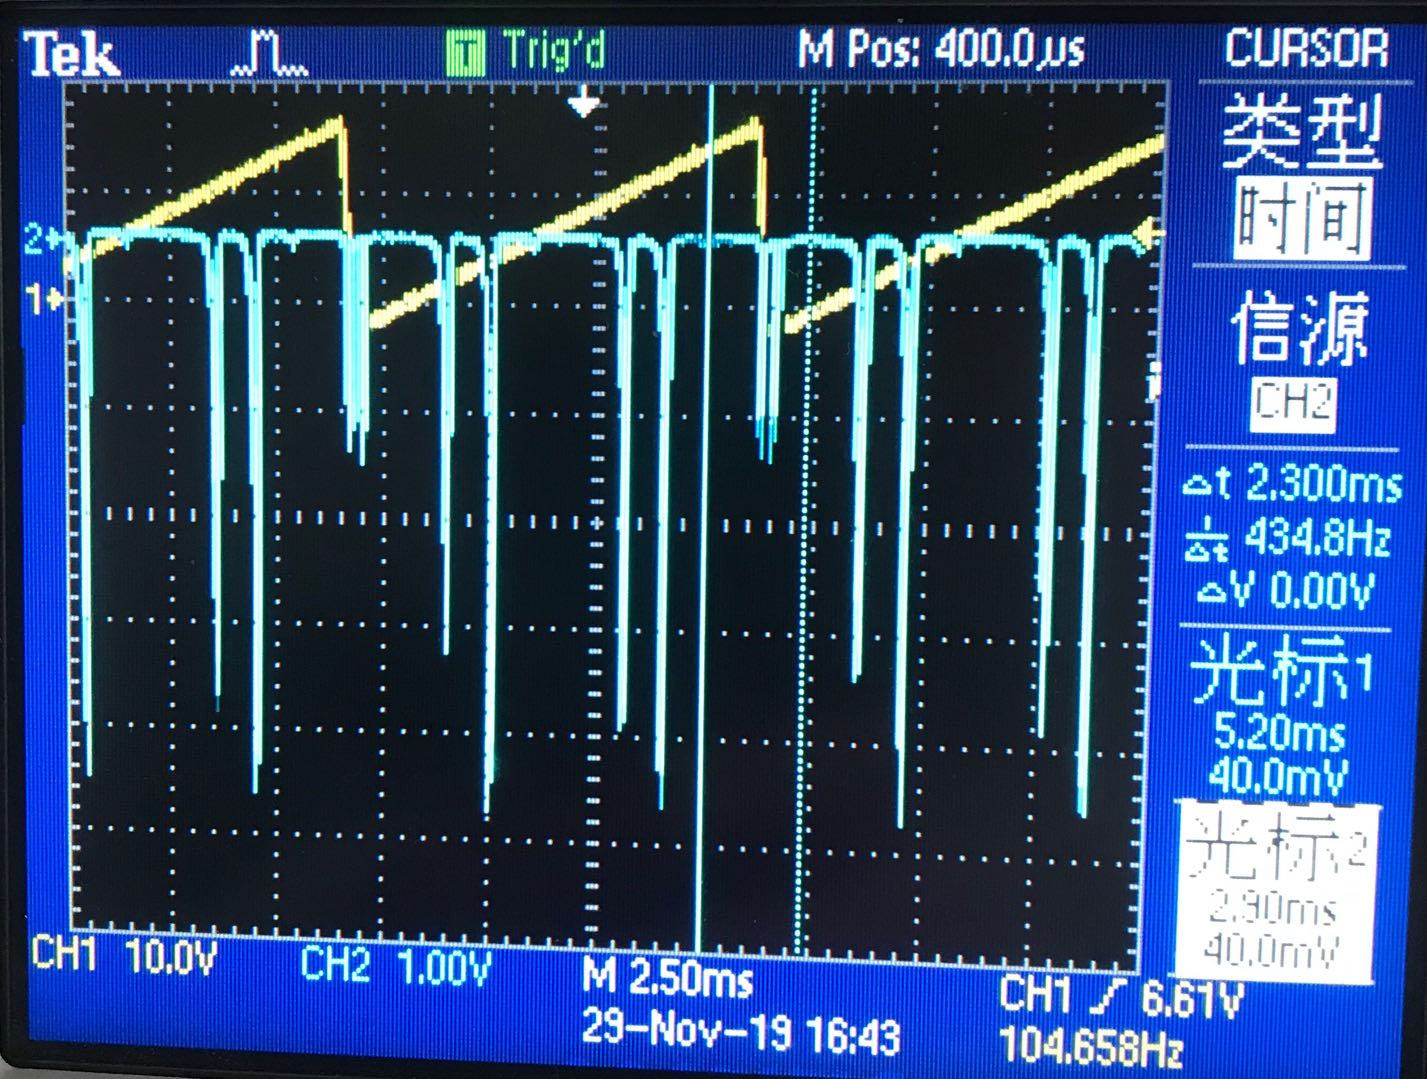
\includegraphics[width=6cm]{short-lengthways}
\caption{短管模谱图}
\end{figure}

观察模谱,可知有两个纵模,测得$\Delta t=0.920ms$,由自由光谱区大小可计算得
\newline$\Delta \nu_{\mbox{纵}}=0.920ms\times\frac{2667MHz}{4.04ms}=607.34MHz$

误差为$(619.83-607.34)/619.83\times100\%=2.0\%$。

短管不存在横模。

\subsection{出光带宽观测}
激光管长$L=284mm$,自由光谱区为$2667MHz$,测得$\Delta t=3.88ms$。出光宽带测得$\Delta t=1.600ms$,计算得$\Delta \nu_=1.600ms\times\frac{2667MHz}{3.88ms}=1099.8MHz$。
取其中三个点测得激光光强对应的感应电压
\begin{table}[H]
\centering
\tiny
\begin{tabular}{|l|l|l|l|}
\hline
$\Delta t/ms$ & 0.36 & 0.72 & 1.2  \\ \hline
$\Delta U/V$  & 6.16 & 8.24 & 3.84 \\ \hline
\end{tabular}
\end{table}
绘得增益曲线
\begin{figure}[H]
\centering
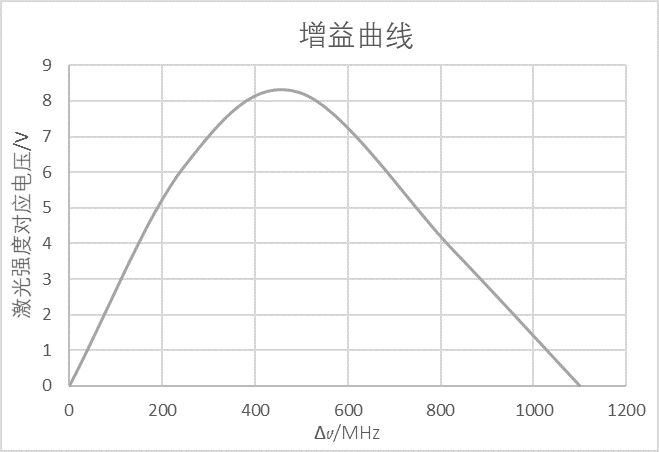
\includegraphics[width=6cm]{u-v}
\end{figure}

\subsection{模分裂}
旋转石英晶体时,观测到模分裂
\begin{figure}[H]
\centering
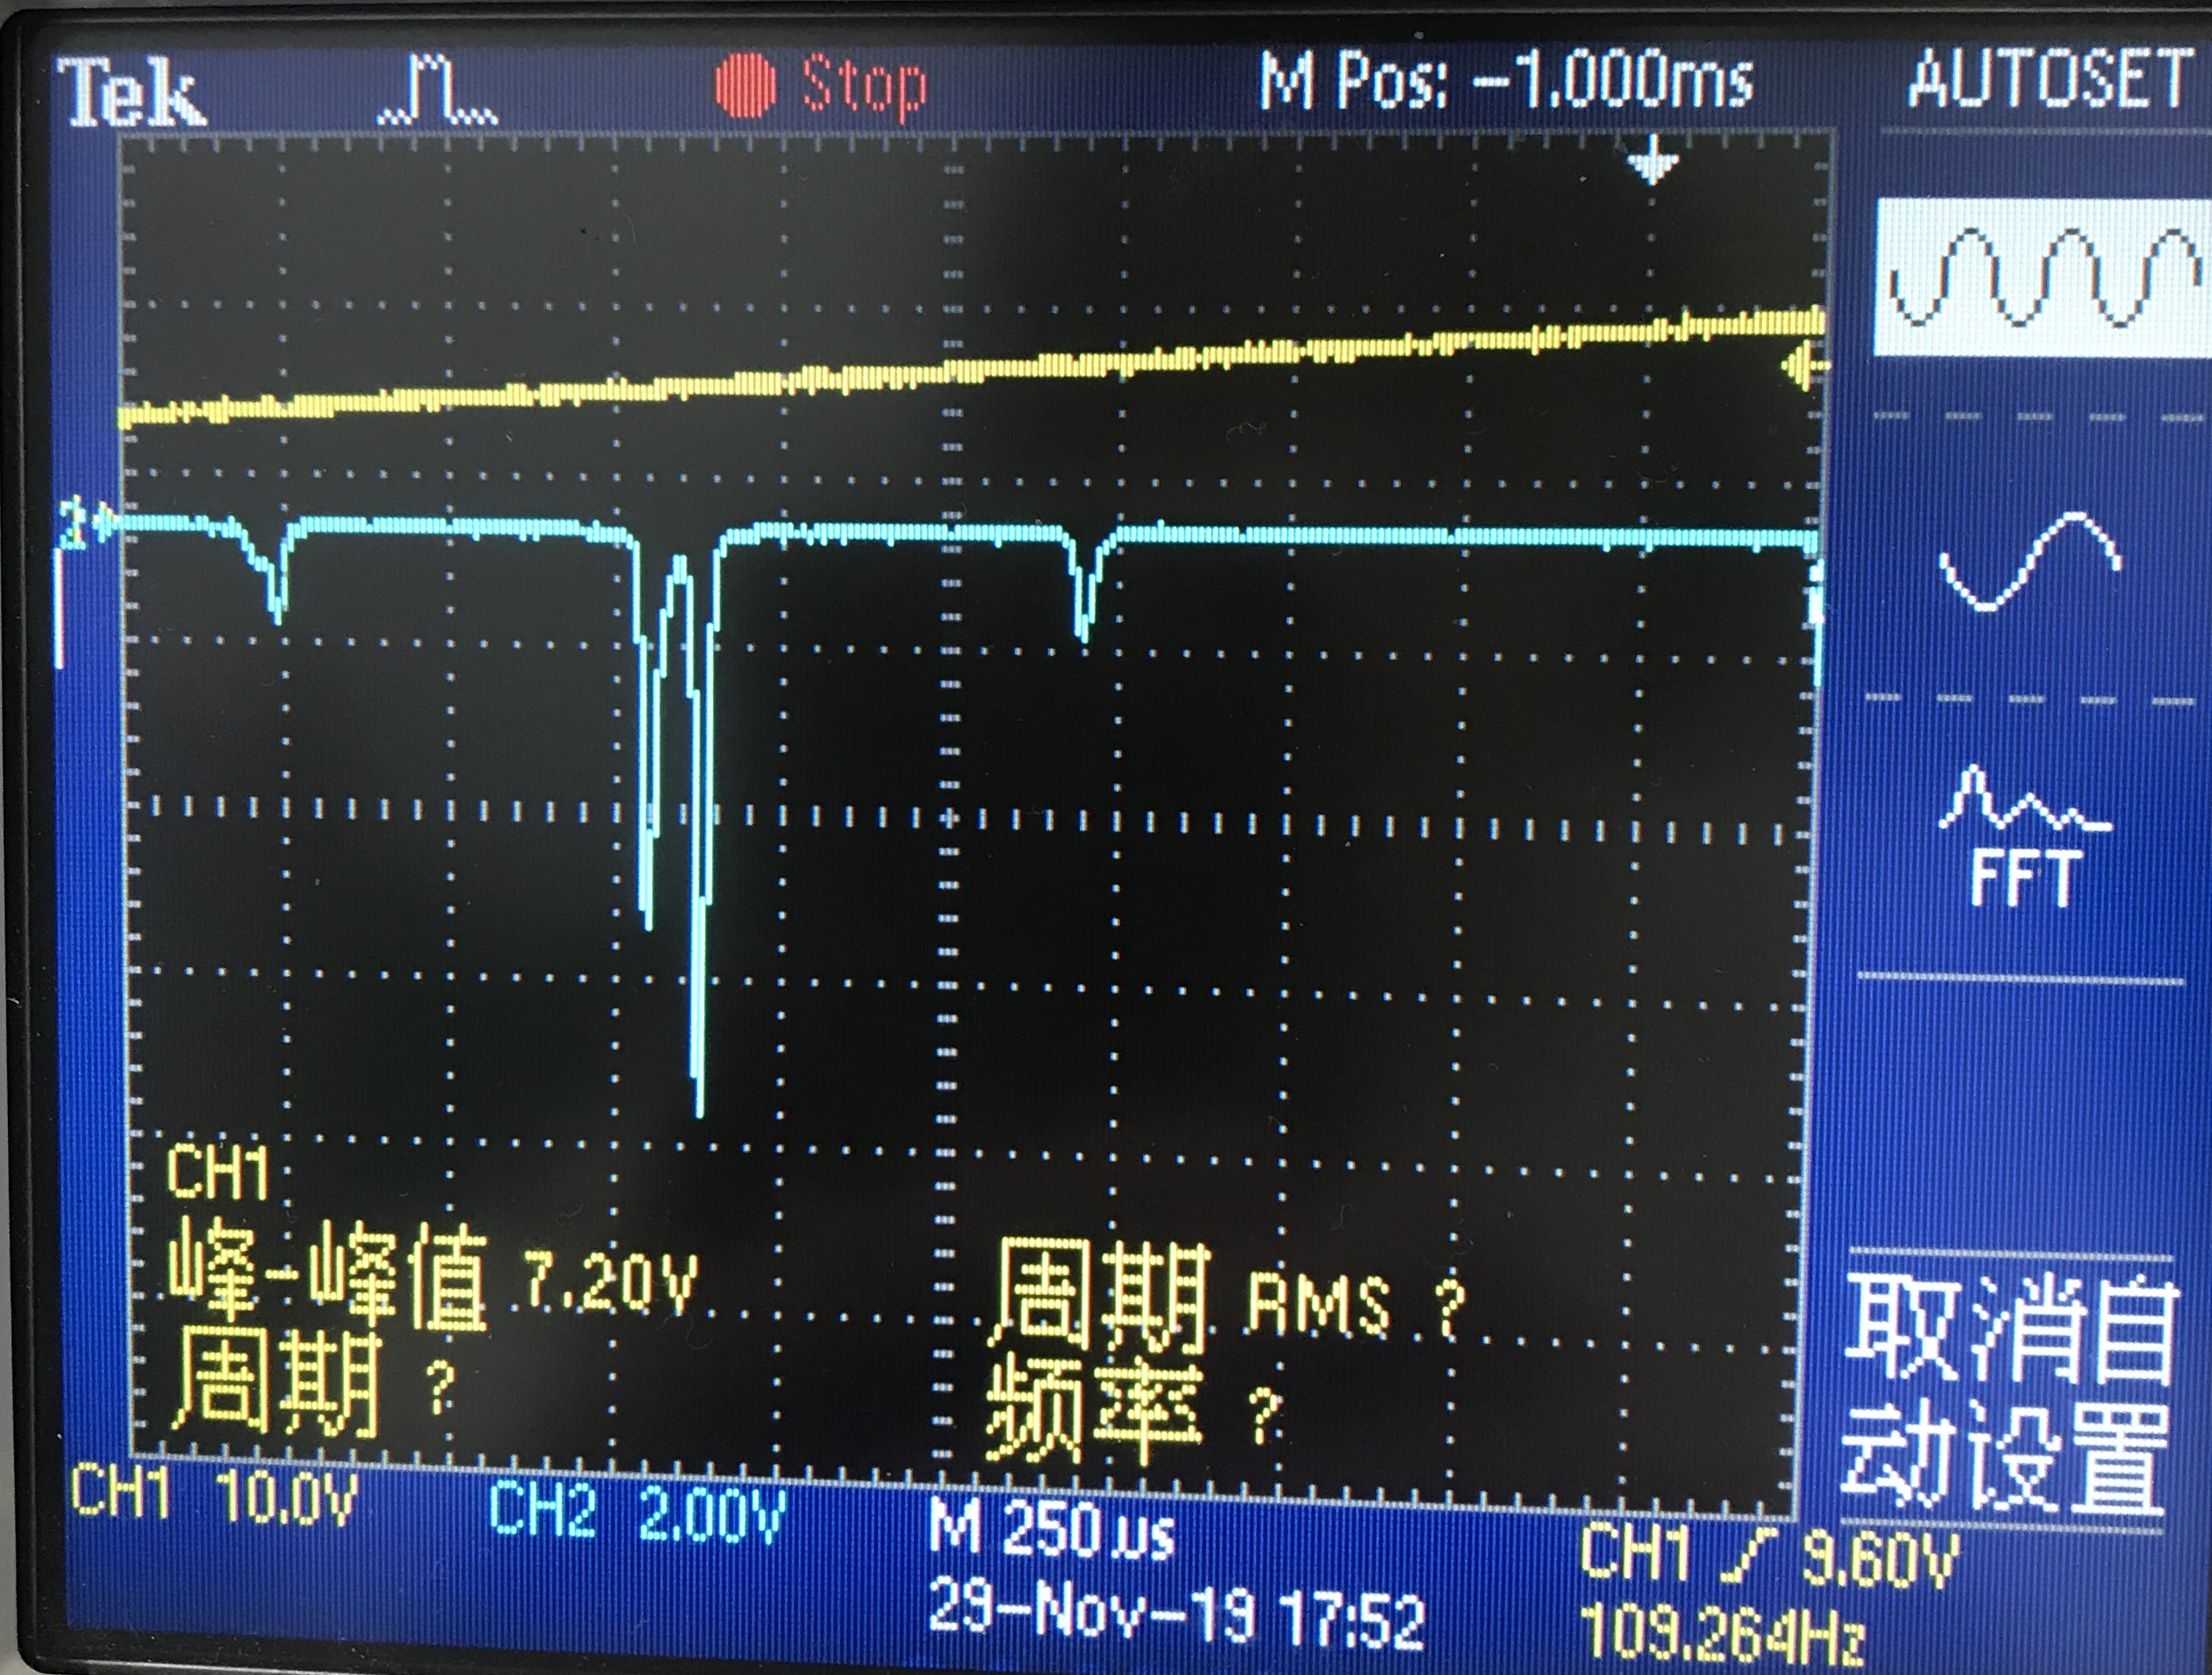
\includegraphics[width=6cm]{seperate}
\end{figure}

用偏振片旋转观测到当一个波长的光强增大时,另一波长的光强减小;直到达到光强极大值,又光强又减小,另一波长同时达到极小值,并光强开始增大。说明这两束光的偏振方向正交。可见是由于石英晶体对o光和e光的双折射现象,产生了模分裂现象。

\section{误差分析}
由于是由人眼定标,且示波器的扫描频率有限,光路未必足够对准,因此造成测量的$\Delta t$存在一定误差。

\section{结论}
激光谐振腔有本征频率,每一个频率对应一种光场分布,叫做一种模式,可以用纵模和横模来完整地描述出来。利用共焦球面扫描干涉仪可以得到激光器出射光的模谱,并对出射光的横、纵模对应的频率间隔进行计算。

由于增益介质的存在,在激光谐振腔中反射时增益大于损耗的频率的光才能出射,故激光器只能出射一定频率的光,这个频率范围就是出光带宽,增益介质有对应的增益曲线。

石英晶体的双折射现象可以使发生模分裂。

\end{multicols}

\section{参考文献}
\small
\noindent[1]北师大物理实验教学中心,近代物理实验2讲义p17-24,2019.

~\\
~\\

\begin{figure}[H]
\centering
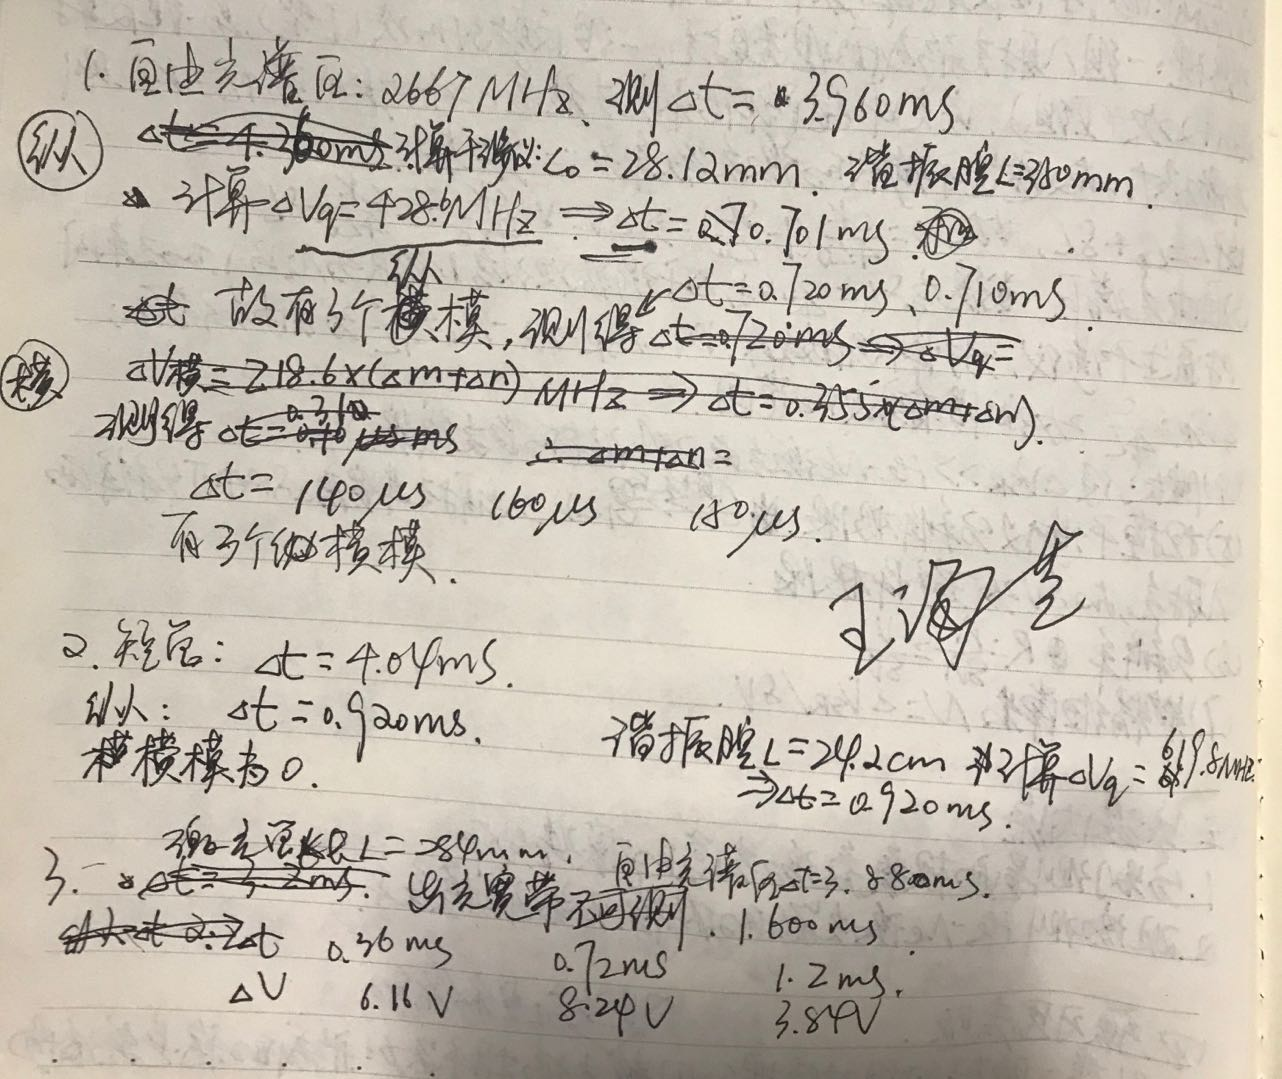
\includegraphics[width=14cm]{statistic}
\end{figure}

\end{document}